\chapter{図表の配置}
\label{ch:figure_table}

\LaTeX で図や表を挿入するときのコマンドは初心者には覚えにくいです.
また,インターネットで検索したものを継ぎ接ぎした結果,何が何だかよくわからないコードができあがるということがよく起きるのでこのファイルからコピーアンドペーストすれば問題ないようにしておきました.
\textcolor{red}{この章ではわかりやすくするために図表のキャプションを全て日本語で書いていますが,実際に学位論文を書く際は全て英語で書いてください.}

\section{図の配置}
\label{sec:figure}

\subsection{図を1枚だけ配置する方法}
\label{ssec:figure_sigle}

ここでは図を1枚だけ配置する方法を紹介します.
図を配置するときは \verb|figure| 環境で図を自動配置し,\verb|\includegraphics| で図を挿入します(図~\ref{fig:one_figure}のコードを参照).
\verb|figure| のオプション \verb|[]| の中にある文字は出力する場所を示します.
\begin{itemize}
    \item \verb|t|\quad ページ上部(\textbf{t}op)に図を出力
    \item \verb|b|\quad ページ下部(\textbf{b}ottom)に図を出力
    \item \verb|p|\quad 単独ページ(\textbf{p}age)に図を出力
    \item \verb|h|\quad できるだけその位置(\textbf{h}ere)に図を出力
    \item \verb|H|\quad 必ずその位置(\textbf{H}ere)に図を出力(\verb|float| パッケージを必要とする)
\end{itemize}
学位論文中の図は原則ページ上部に配置するのでこの \verb|tex| ファイル中では \verb|[tp]| に設定してあります.
皆さんはこのままコピーしてください.
\verb|\columnwidth| は現在のコラムのテキスト幅を指しており,\verb|[width=0.5\columnwidth]| と設定することで,テキスト幅の半分の横幅で図を挿入できます.
図の大きさの指定に関してよく使うコマンドをテキストボックスにまとめてあります.
\verb|\textwidth|,\verb|\columnwidth|,\verb|\linewidth| はよく似たコマンドですが,二段組の論文の場合はそれぞれの段の列幅が \verb|\columnwidth| になり,\verb|\linewidth| はリストなどの環境下での行の長さで臨機応変に対応します.
これらは文書内のある長さに対して相対的に図の大きさを決定する方法でしたが,\verb|width=25mm| のように絶対的な長さも指定できます.
\verb|\centering| は図を中央寄せするコマンドです\footnote{図などを中央寄せする際に \texttt{\textbackslash begin\{center\}} で始まる \texttt{center} 環境を使うのは非推奨です.}.

また,コードにもあるように \verb|\label{}| コマンドを挿入することでラベルを設定できます.
ここでは \verb|\label{fig:one_figure}| としており,ラベル参照時に図であることがわかるよう \verb|fig:| を入れています.
ご自身の論文の内容に合わせてキャプションやラベルは変更してください.
文章中で引用する際は \verb|図~\ref{fig:one_figure}| のように書きます.
すると図~\ref{fig:one_figure}のように出力されます.
ハイパーリンクも埋め込まれているので該当する図が遠く離れた位置にあっても便利です.
ここで「図」と番号の間にチルダ \verb|~| を入れているのはここでの改行を防止を目的としています.

\begin{tcolorbox}[enhanced, title={\texttt{\textbackslash includegraphics} で図の大きさの指定によく使うコマンド}, drop fuzzy shadow]
    【指定するもの】

    \begin{tabular}{lll}
        コマンド    & 意味  & 使用例 \\
        \verb|width|    & 画像の幅          & \verb|width=0.5\textwidth| \\
        \verb|height|   & 画像の高さ        & \verb|height=0.1\textheight|\\
        \verb|scale|    & 画像のスケール    & \verb|scale=0.5|
    \end{tabular}

    【長さに関するコマンド】

    \begin{tabular}{ll}
        コマンド   & 意味 \\
        \verb|\textwidth|   & テキストエリアの幅 \\
        \verb|\textheight|  & テキストエリアの高さ \\
        \verb|\columnwidth| & テキスト列の幅 \\
        \verb|\linewidth|   & 現在の環境内での行の長さ
    \end{tabular}
\end{tcolorbox}

%%% 図を 1 枚だけ配置するときはこれをコピーアンドペーストすればよい.
\begin{figure}[tp]
    \centering
    
\includegraphics[width=0.5\columnwidth]{figure/tiger.pdf}
    \caption{1枚の図.}
    \label{fig:one_figure}
\end{figure}
%%%

\subsection{図を複数枚配置する方法}
\label{ssec:multiple}

関連する図(ここではそれぞれの図を「サブ図」と呼称します)を複数枚配置するときは \verb|subcaption| を使いましょう\footnote{\texttt{subfigure} や \texttt{subfig} は古いので非推奨です.}.
このテンプレートでは \verb|settings.sty| 内で読み込んでいます.
文章中では \verb|subfigure| 環境に入れて並べます.
例えば 2 枚の図を横に並べて配置したいときは図~\ref{fig:two_figures}のようになります.
ここでは \verb|\hfill| を使って図と図の間の空白を設定していますが,\verb|\hspace{3mm}| のように設定しても構いません.
\verb|\hspace{3mm}| の場合,水平方向に$\SI{3}{\milli\meter}$の空白ができます.
3 枚のサブ図を横に並べたいときも同様で,図~\ref{fig:three_figures}のようになります.
関連するサブ図を横だけでなく縦方向にも配置したいときは,図~\ref{fig:four_figures}のように横並びの \verb|\columnwidth| の合計が大きくなりすぎると自動的に縦に配列してくれます.
ここでは縦方向のスペースを確保するために \verb|\vspace{5mm}| を挿入しています.

\begin{tcolorbox}[enhanced, title={図のラベルの参照方法}, drop fuzzy shadow]
    \begin{tabular}{ll}
        入力     & 出力 \\
        \verb|\ref{fig:one_figure}|                                                 & \ref{fig:one_figure} \\
        \verb|\ref{fig:two_figures}|                                                & \ref{fig:two_figures} \\
        \verb|\ref{subfig:two_figures_a}|                                           & \ref{subfig:two_figures_a} \\
        \verb|\ref{fig:two_figures}(\subref{subfig:two_figures_a})|                 & \ref{fig:two_figures}(\subref{subfig:two_figures_a}) \\
        \verb|(\subref{subfig:two_figures_a}, \subref{subfig:two_figures_b})|       & (\subref{subfig:two_figures_a}, \subref{subfig:two_figures_b}) \\
        \verb|(\subref{subfig:four_figures_a}--\subref{subfig:four_figures_c})|    & (\subref{subfig:four_figures_a}--\subref{subfig:four_figures_c})
    \end{tabular}
\end{tcolorbox}

また,\verb|subfigure| 環境を使うことでそれぞれのサブ図にラベルを付けることができます.
参照時には \verb|\ref{fig:two_figures}| と入力すると \ref{fig:two_figures} のように図全体の番号のみ,\verb|\subref{subfig:four_figures_a}| と入力すると \subref{subfig:two_figures_a} のようにサブ図の番号のみ出力されます.
図~\ref{fig:two_figures} のように出力したい場合は \verb|図~\ref{fig:two_figures}| とすればよいですが,仮に図~\ref{fig:two_figures}(\subref{subfig:two_figures_a}) のように出力したい場合は \verb|図~\ref{fig:two_figures}(\subref{subfig:two_figures_a})| とします.
このとき,\verb|\subref{}| 前後の括弧 \verb|()| を忘れないでください.
仮に \verb|\ref{subfig:two_figures_a}| のようにサブ図を \verb|\ref{}| コマンドで直接指定してあげると \ref{subfig:two_figures_a} のように図番号とサブ図番号が括弧無しで出力されます.
括弧をデフォルトで出力するような設定もできますが,図~\ref{fig:two_figures}(\subref{subfig:two_figures_a}, \subref{subfig:two_figures_b}) や図~\ref{fig:four_figures}(\subref{subfig:four_figures_a}--\subref{subfig:four_figures_c}) のように複数のサブ図を指定するときに不便なので括弧を外してあります.
もしデフォルトで括弧を出力する設定に変更したい場合は \verb|settings.sty| 内でコメントアウトしている \verb|\renewcommand{\thesubfigure}{(\alph{subfigure})}| を有効化してください.




%%% 図を 2 枚横並びで配置するときはこれをコピーアンドペーストすればよい.
\begin{figure}[tp]
    \centering
    \begin{subfigure}{0.45\columnwidth}
        \centering
        \includegraphics[width=\columnwidth]{example-image-a}
        \caption{左の図.}
        \label{subfig:two_figures_a}
    \end{subfigure}
    \hfill % ここで空白を入れると図が適切に配置される
    \begin{subfigure}{0.45\columnwidth}
        \centering
        \includegraphics[width=\columnwidth]{example-image-b}
        \caption{右の図.}
        \label{subfig:two_figures_b}
    \end{subfigure}
    \caption{左右の図.}
    \label{fig:two_figures}
\end{figure}
%%%

%%% 図を 3 枚横並びで配置するときはこれをコピーアンドペーストすればよい.
\begin{figure}[tp]
    \centering
    \begin{subfigure}{0.32\columnwidth}
        \centering
        \includegraphics[width=\columnwidth]{example-image-a}
        \caption{左の図.}
        \label{subfig:three_figures_a}
    \end{subfigure}
    \hfill % ここで空白を入れると図が適切に配置される
    \begin{subfigure}{0.32\columnwidth}
        \centering
        \includegraphics[width=\columnwidth]{example-image-b}
        \caption{中央の図.}
        \label{subfig:three_figures_b}
    \end{subfigure}
    \hfill % ここで空白を入れると図が適切に配置される
    \begin{subfigure}{0.32\columnwidth}
        \centering
        \includegraphics[width=\columnwidth]{example-image-c}
        \caption{右の図.}
        \label{subfig:three_figures_c}
    \end{subfigure}
    \caption{3枚の図.}
    \label{fig:three_figures}
\end{figure}
%%%

%%% 図を 4 枚上下左右に配置するときはこれをコピーアンドペーストすればよい.
\begin{figure}[tp]
    \centering
    % 上の行
    \begin{subfigure}{0.45\columnwidth}
        \centering
        \includegraphics[width=\columnwidth]{example-image-a}
        \caption{左上の図.}
        \label{subfig:four_figures_a}
    \end{subfigure}
    \hfill % 水平方向のスペース
    \begin{subfigure}{0.45\columnwidth}
        \centering
        \includegraphics[width=\columnwidth]{example-image-b}
        \caption{右上の図.}
        \label{subfig:four_figures_b}
    \end{subfigure}

    \vspace{5mm} % 縦方向のスペース
    % 下の行
    \begin{subfigure}{0.45\columnwidth}
        \centering
        \includegraphics[width=\columnwidth]{example-image-c}
        \caption{左下の図.}
        \label{subfig:four_figures_c}
    \end{subfigure}
    \hfill % 水平方向のスペース
    \begin{subfigure}{0.45\columnwidth}
        \centering
        \includegraphics[width=\columnwidth]{example-image-c}
        \caption{右下の図.}
        \label{subfig:four_figures_c2}
    \end{subfigure}
    \caption{上下左右に4つ配置した図.}
    \label{fig:four_figures}
\end{figure}
%%%

\clearpage
\subsection{画像のファイル形式}
\label{ssec:figure_format}

画像形式は大きく分類するとラスター画像とベクター画像に分類できます.
結論から先に述べると,\textcolor{red}{ラスター画像であれば JPEG か PNG,ベクター画像であれば PDF を使用してください}.

\begin{itemize}
    \item ラスター画像:小さな正方形(ピクセル,画素)を大量に組み合わせて作り上げた画像.ラスター画像を拡大するとピクセルの存在を確認できる.ラスター画像の例は以下の通り.
    \begin{itemize}
        \item GIF (Graphics Interchange Format):拡張子は \verb|.gif| で,256 色以下の画像を扱える可逆圧縮形式ファイル.使用できる色は少ないものの,アニメーションにも対応していることから現在でも使う機会が多い.
        \item JPEG (Joint Photographic Experts Group):拡張子は \verb|.jpeg| や \verb|.jpg| で,最大 24 ビット(約 1677 万色)の色に対応している非可逆圧縮形式ファイル.
        \item PNG (Portable Network Graphics):拡張子は \verb|.png| で,JPEG と同様 24 ビットの色に対応している可逆圧縮形式ファイル.透過処理にも対応している.
    \end{itemize}
    \item ベクター画像:円や直線などを数式的に処理することで作り上げた画像.どれだけ拡大しても明瞭なまま.ベクター画像の例は以下の通り,
    \begin{itemize}
        \item PS (PostScript):拡張子は \verb|.ps| で,Adobe が 1984 年に開発したページ記述言語で組まれた画像形式.
        \item EPS (Encapsulated PostScript):拡張子は \verb|.eps| で,PostScript の後継となる画像形式(カプセル化された PostScript).バウンディングボックスを読み込むことで描画領域を確保する.
        \item PDF (Portable Document Format):拡張子は \verb|.pdf| で,環境に左右されず,ほぼ同様の見た目で画像や文書を閲覧できる.一般的な用途では最も主流なベクター形式.
    \end{itemize}
\end{itemize}

ラスター画像かベクター画像かという観点では,論文中の画像はできるだけベクター画像の方がいいです.
これは上記説明にも書いたように,ベクター画像は内部で数式処理をしているためいくら拡大しても解像度が落ちず明瞭なままだからです.
ただし,これは一般的なグラフや簡単なカラーマップ限定の話です.
複雑なカラーマップをベクター画像にするとファイルサイズが膨大になり,画像を開くだけでも一苦労です.
このような場合には諦めてラスター画像にしましょう.

また,一昔前の \LaTeX では画像の挿入と言えば EPS ファイルでした.
しかし,現在の \LaTeX 事情では EPS ファイルの使用は非推奨です.
本来 \TeX エンジンは EPS ファイルを直接処理することができず,Ghostscript という PostScript 言語のインタープリターを経由しなければいけません.
したがって,最初から PDF で挿入する方がよいというわけです.
また,バウンディングボックスの調節がうまくいかず,EPS で挿入すると画像がずれるという問題が生じることがあります.
現代に生きる皆さんは EPS ではなく PDF を使いましょう.

\begin{figure}[tp]
    \centering
    % 上の行
    \begin{subfigure}{0.45\columnwidth}
        \centering
        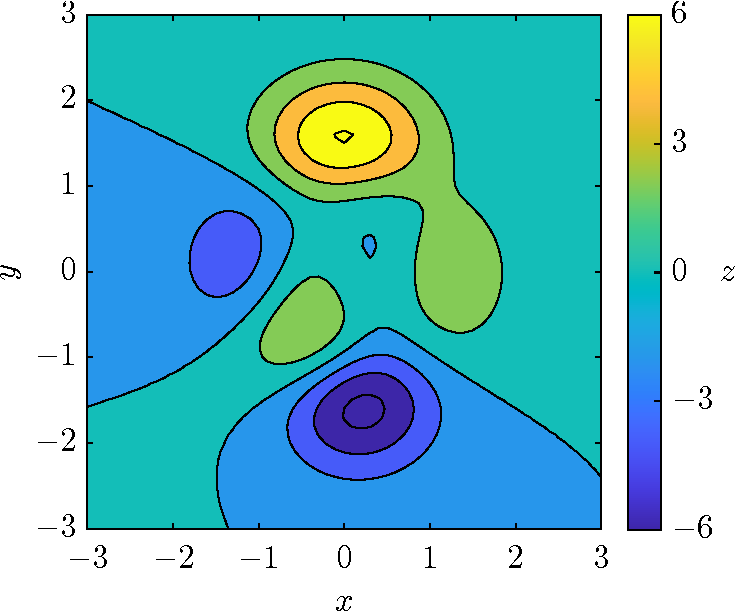
\includegraphics[width=\columnwidth]{figure/comparison1-1.pdf}
        \caption{PDF ファイル(文字抽出可).}
        \label{subfig:figcomp1_pdf}
    \end{subfigure}
    \hfill % 水平方向のスペース
    \begin{subfigure}{0.45\columnwidth}
        \centering
        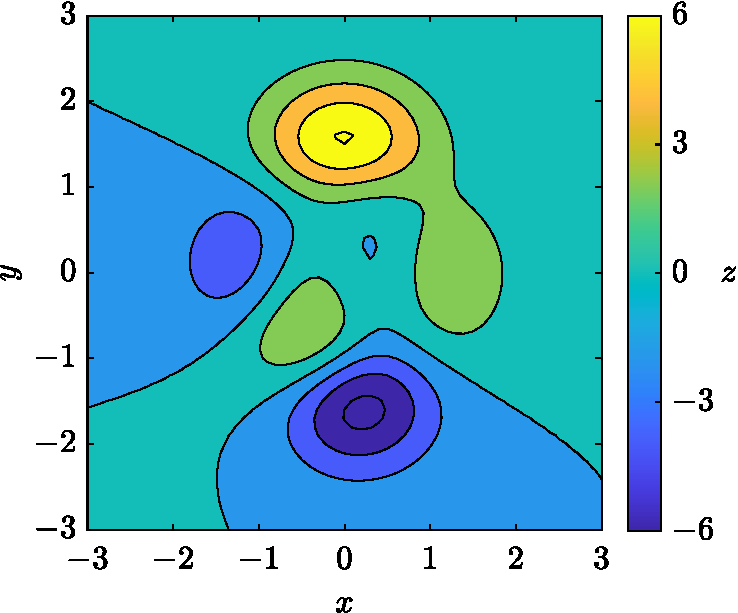
\includegraphics[width=\columnwidth]{figure/comparison1-2.pdf}
        \caption{PDF ファイル(文字抽出不可).}
        \label{subfig:figcomp1_pdf2}
    \end{subfigure}

    \vspace{5mm} % 縦方向のスペース
    % 下の行
    \begin{subfigure}{0.45\columnwidth}
        \centering
        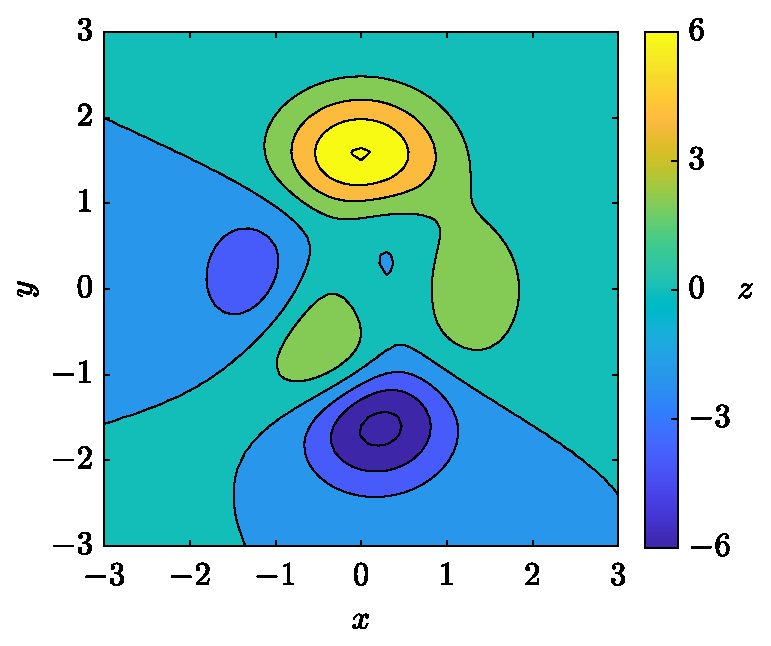
\includegraphics[width=\columnwidth]{figure/comparison1-3.eps}
        \caption{EPS ファイル.}
        \label{subfig:figcomp1_eps}
    \end{subfigure}
    \hfill % 水平方向のスペース
    \begin{subfigure}{0.45\columnwidth}
        \centering
        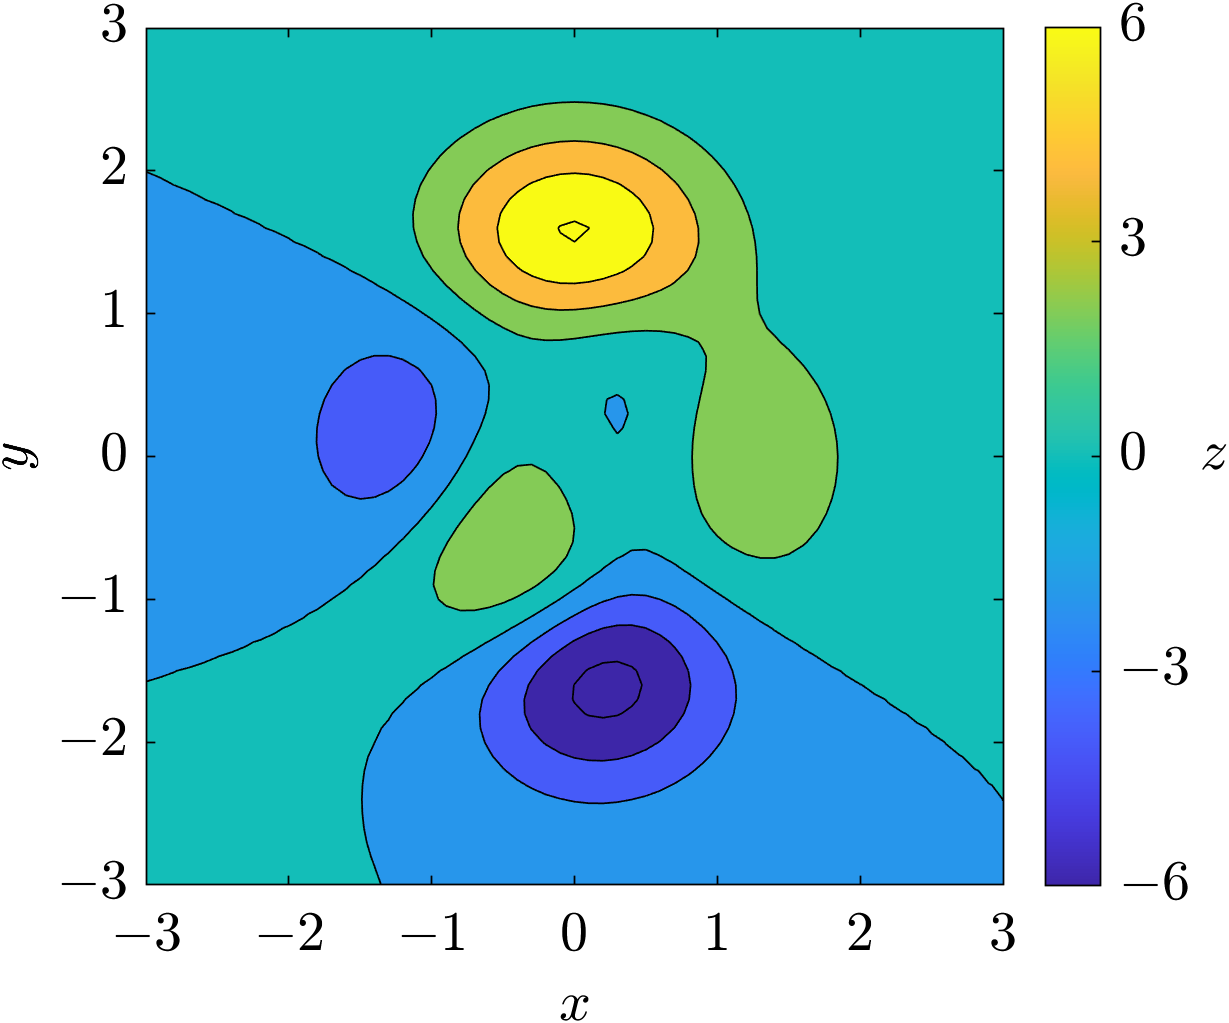
\includegraphics[width=\columnwidth]{figure/comparison1-4.png}
        \caption{PNG ファイル.}
        \label{subfig:figcomp1_png}
    \end{subfigure}
    \caption{画像形式ごとの比較.}
    \label{fig:figure_comparison1}
\end{figure}

それでは実際にいくつかの画像形式を比較してみましょう.
図~\ref{fig:figure_comparison1} では (\subref{subfig:figcomp1_pdf}, \subref{subfig:figcomp1_pdf2}) PDF ファイル,(\subref{subfig:figcomp1_eps}) EPS ファイル,(\subref{subfig:figcomp1_png}) PNG ファイルを並べて比較しています.
パネル~(\subref{subfig:figcomp1_pdf}--\subref{subfig:figcomp1_eps}) はどれもベクター画像なのでいくら拡大しても明瞭なままですね.
一方のパネル~(\subref{subfig:figcomp1_png}) を拡大するとラスター画像なので小さな正方形で構成されていることが確認できます.
これがベクター画像とラスター画像の違いです.
それではパネル~(\subref{subfig:figcomp1_pdf}) と (\subref{subfig:figcomp1_pdf2}) の違いは何でしょうか.
どちらも PDF 形式ですよね.
\verb|main.pdf| を開きながら \verb|Ctrl|+\verb|A| をしてください.
パネル~(\subref{subfig:figcomp1_pdf}) は文字を抽出できますが,(\subref{subfig:figcomp1_pdf2}) は文字を抽出できません.
皆さんが論文を書く際は (\subref{subfig:figcomp1_pdf}) 文字抽出が可能な PDF を使用するのが理想です.

\begin{figure}[tp]
    \centering
    \begin{subfigure}{0.45\columnwidth}
        \centering
        \includegraphics[height=0.26\textheight]{figure/comparison2-1.pdf}
        \caption{PDF ファイル.}
        \label{subfig:figcomp2_pdf}
    \end{subfigure}
    \hspace{3mm} % ここで空白を入れると図が適切に配置される
    \begin{subfigure}{0.45\columnwidth}
        \centering
        \includegraphics[height=0.26\textheight]{figure/comparison2-2.png}
        \caption{PNG ファイル.}
        \label{subfig:figcomp2_png}
    \end{subfigure}
    \caption{ファイルサイズが大きい画像の比較.}
    \label{fig:figure_comparison2}
\end{figure}

ただし,全ての画像をベクター画像にするのは難しい場合もあります.
図~\ref{fig:figure_comparison1} の場合はファイルサイズの小さいカラーマップだったのでベクター画像として貼っても問題ありませんが,もっと複雑な模様だととても扱えるようなファイルサイズではありません.
図~\ref{fig:figure_comparison2}(\subref{subfig:figcomp2_pdf}) はカラーマップだけラスターとし,文字情報は全てベクターで抽出できるようになっています(ファイル自体は PDF).
パネル~(\subref{subfig:figcomp2_png}) は全てラスターの画像(PNG)なので文字を抽出することはできません.
ただ,図~\ref{fig:figure_comparison2}(\subref{subfig:figcomp2_pdf}) のような図を作るのは少し技術を要するので,重い画像ファイルの場合は (\subref{subfig:figcomp2_png}) のようなラスター画像でもいいでしょう.


\section{表の配置}
\label{sec:table}

次に表の作り方を説明します.
正直,\LaTeX 環境での表作成は少々面倒です.
特に表のセルの数が多くなると行をいくつも増やさなければいけないのでかなりの労力がかかります.
簡単に \LaTeX の表を作ってくれるツールとして,Tables Generator\footnote{Tables Generator, \textless\url{https://www.tablesgenerator.com/}\textgreater} があります.
また,\href{https://www.overleaf.com/blog/major-feature-news-add-and-edit-tables-without-writing-code}{2023 年 9 月 27 日に Overleaf に入ったアップデート}で直感的な表の作成が可能になりました.
Overleaf の表作成機能はかなり便利だと思うので,ローカルで \LaTeX 文書を書いているときに表作成時だけでも Overleaf を立ち上げるとストレス無く表を作れると思います.

ここでは \verb|tabular| 環境を用いた表作成の方法と \verb|tblr| 環境を用いた表作成の方法の両方を記載します.
\verb|tabular| 環境は古くから存在している表作成の方法ですが,カスタマイズ性が低く,非常に使いにくいです.
しかし,\verb|tabularray| パッケージ\footnote{\LaTeX3 を利用した新しいパッケージです.}でサポートされている \verb|tblr| 環境は非常にカスタマイズ性が高く,\verb|tabular| 環境で非常に難しかったセル結合も容易に行えます.
\verb|tabluar| 環境は現在でも広く使われているためこのテンプレートでも説明しますが,皆さんが論文を書くときは是非 \verb|tblr| 環境を使ってみてください.

\subsection{\texttt{tabular} 環境を用いた表}
\label{ssec:tabular}

%%% tabular 環境を用いた表のサンプルコード
\begin{table}[tp]
    \centering
    \caption{\texttt{tabular} 環境を用いた表のサンプル.}
    \label{table:tabular}
    \begin{tabular}{l|c|r} \hline\hline
        \multicolumn{1}{c|}{学会名}  & 会員種別  & \multicolumn{1}{c}{年会費} \\ \hline
        \multicolumn{3}{c}{実在する学会} \\ \hline
        日本機械学会    & 学生員    & 4,800 円 \\ \hline
        日本流体力学会  & 学生会員  & 5,000 円 \\ \hline
        日本伝熱学会    & 学生会員  & 4,000 円 \\ \hline
        \multicolumn{3}{c}{実在しない学会} \\ \hline
        \multirow{4}{*}{日本架空学会}& 小学生会員  & $-8,000$ 円 \\ \cline{2-3}
        & 中高生会員  & $-5,000$ 円 \\ \cline{2-3}
        & 大学生会員  & $-2,000$ 円 \\ \cline{2-3}
        & 名誉学生会員  & $6.02 \times 10^{23}$ 円 \\ \hline
    \end{tabular}
\end{table}
%%%

日本機械学会が推奨する表形式を満たしたサンプルを表~\ref{table:tabular} に示します.
コードは表~\ref{table:tabular} の該当箇所を確認してください.
表を作成するときは \verb|table| 環境の中に \verb|tabular| 環境を作ります.
\verb|table| 環境は,表やキャプション,ラベルを全て含めた表全体の制御を行い,\verb|tabular| 環境は表の各セルの制御を行います.
\verb|table| 環境は \verb|figure| 環境と同様,\verb|h|, \verb|t|, \verb|b|, \verb|p|, \verb|H| による位置制御を行います.
表の場合は図と異なり,キャプションは上に付けます.
\verb|tabular| 環境内でセルの文字揃え位置制御は \verb|lcr| で行います.

\begin{itemize}
    \item \verb|l|\quad 左揃え(\textbf{l}eft)
    \item \verb|c|\quad 中央揃え(\textbf{c}enter)
    \item \verb|r|\quad 右揃え(\textbf{r}ight)
\end{itemize}

表~\ref{table:tabular} の場合は \texttt{\{l|c|r\}} としています.
この場合,左の列から左寄せ・中央寄せ・右寄せになります.
縦棒(バーティカルライン)\verb||| は表の縦罫線を入れる場所を示しています.
この場合,1 列目と 2 列目の間,2 列目と 3 列目の間に縦罫線を入れます.
行の区切りは \verb|\\|,列の区切りは \verb|&| です.
横罫線を引くときは \verb|\hline| を使います.
日本機械学会のテンプレートの表では一番上の横罫線は 2 本なので \verb|\hline\hline| としています.

次に表のセル結合について説明します.
行方向のセル結合を行う際は \verb|\multicolumn{結合する列数}{揃え位置}{セルの中身}| を使います(結合するセルは列).
表~\ref{table:tabular} の 2 行目で使用している \verb|\multicolumn{3}{c}{実在する学会}| は「横並びの 3 つのセルを結合し,『実在する学会』という文字列を中央揃えで配置する」命令です.
1 行 1 列目では \texttt{\textbackslash multicolumn\{1\}\{c|\}\{学会名\}} としていますが,これは本来左揃えになっている 1 列目を,このセルだけ例外的に中央揃えにするために使用しています.
面白い使い方ですね.
列方向のセル結合を行う際は \verb|\multirow{結合する行数}{幅}{セルの中身}| を使います(結合するセルは行).
表~\ref{table:tabular} の 7 行 1 列目で使用している \verb|\multirow{4}{*}{日本架空学会}| は「縦並びの 4 つのセルを結合し,『日本架空学会』という文字列を幅指定なしで配置する」命令です.
列方向のセル結合を行う際は横罫線を消す必要があります.
\verb|\cline{x-y}| という命令を使うと,x 列目から y 列目に横罫線を入れるコマンドです.
\verb|\hline| がその行全体に横罫線を入れるのに対して \verb|\cline{}| はその行に部分的な横罫線を入れるコマンドです.
横罫線を消すことでセル結合したような出力を得られます.

\begin{tcolorbox}[enhanced, title={\texttt{tabular} 環境でセル結合する際に使用するコマンド}, drop fuzzy shadow]
    \begin{tabular}{ll}
        \verb|\multicolumn{結合する列数}{揃え位置}{セルの中身}| & 列のセル結合  \\
        \verb|\multirow{結合する行数}{幅}{セルの中身}|  & 行のセル結合  \\
        \verb|\cline{start-end}|    & 一部の横罫線のみを表示
    \end{tabular}
\end{tcolorbox}

また,表の中では数式を使用することも可能です.
やりがちなミスとして,負の数をセルに入れるときに数式環境 \verb|$$| に入れ忘れて,マイナスがハイフンとなって出力されているものがあります\footnote{例えば $-100$ と表示するには \texttt{\$-100\$} と入力する必要があります.\texttt{-100} だと -100 と表示されます.}.


\subsection{\texttt{tblr} 環境を用いた表}
\label{ssec:tblr}

%%% tblr 環境を用いた表のサンプルコード
\begin{table}[tp]
    \centering
    \caption{\texttt{tblr} 環境を用いた表のサンプル.}
    \label{table:tblr}
    \begin{tblr}{
        colspec = {l|c|r},  % 文字の揃え位置制御
        hlines,             % 横罫線の表示
        % vlines,             % 縦罫線の表示
    } \hline
        \SetCell{c} 学会名  & 会員種別      & \SetCell{c} 年会費 \\
        \SetCell[c=3]{c} 実在する学会   &   &   \\
        日本機械学会       & 学生員        & 4,800 円 \\
        日本流体力学会     & 学生会員      & 5,000 円 \\
        日本伝熱学会       & 学生会員      & 4,000 円 \\
        \SetCell[c=3]{c} 実在しない学会   &   &   \\
        \SetCell[r=4]{l} 日本架空学会   & 小学生会員    & $-8,000$ 円 \\
        & 中高生会員    & $-5,000$ 円 \\
        & 大学生会員    & $-2,000$ 円 \\
        & 名誉学生会員  & $6.02 \times 10^{23}$ 円 \\
    \end{tblr}
\end{table}
%%%

表~\ref{table:tblr} は \verb|tblr| 環境を用いた表のサンプルです.
見た目が表~\ref{table:tabular} と同じになるようにしています.
基本的な使い方は \verb|tabular| 環境に準じています.
大きな違いは罫線の扱いです.
\verb|\begin{tblr}| の直後で \verb|hlines| を入れると全ての横罫線が,\verb|vlines| を入れると全ての縦罫線が表示されます.
また,セル結合の方法も異なります.
表~\ref{table:tblr} の 2 行目の \verb|\SetCell[c=3]{c} 実在する学会| は「横並びの 3 つのセルを結合し,『実在する学会』という文字列を中央揃えで配置する」命令です.
1 行 1 列目では \verb|\SetCell{c} 学会名| とすることでこのセルだけ中央揃えに変えています.
7 行 1 列目の \verb|\SetCell[r=4]{l} 日本架空学会| は「縦並びの 4 つのセルを結合し,『日本架空学会』という文字列を左揃えで配置する」命令です.

\begin{tcolorbox}[enhanced, title={\texttt{tblr} 環境でセル結合する際に使用するコマンド}, drop fuzzy shadow]
    \begin{tabular}{ll}
        \verb|\SetCell{c}|   & そのセルだけ中央揃えに変更 \\
        \verb|\SetCell[r=3]{c}|  & 3 行をセル結合し中央揃え \\
        \verb|\SetCell[c=3]{c}|  & 3 列をセル結合し中央揃え \\
        \verb|\SetCell[r=2,c=3]{c}|  & 2 行 3 列をセル結合し中央揃え \\
    \end{tabular}
\end{tcolorbox}

